\documentclass[./main.tex]{subfiles}

\begin{document}
\section{Improving the Model}\label{sec:improving}
% Mangler intro
\subsection{Motivation}
In Section \ref{sec:XAI} we explored the developed model from Section \ref{experiement}. By doing so we found out, that the latent space of the model has some inconsistency of the placement of the training observations, as well as having some principal components that acts as noise, which could explain the not optimal performance of the model. By helping improving the latent space of the model, as well as removing some of the noise, we could improve the performance of the model, which can be done by making use of an autoencoder.

\subsection{Configuration Details}
\begin{figure}[htbp]
    \centering
    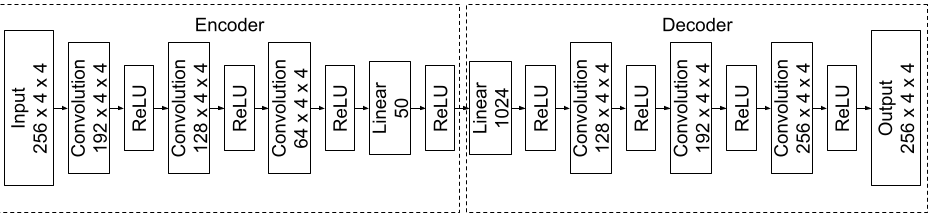
\includegraphics[width = \textwidth]{entities/Ae_model.png}
    \caption{Visualization of the architecture of the developed autoencoder. The numbers in each box represents the dimensions of the output of the corresponding layer.}
    \label{fig:AE_model}
\end{figure}
The developed autoencoder has been visualized in Figure \ref{fig:AE_model}. The autoencoder makes use of convolutional layers and linear layers to downsample the input down to only $50$ dimensions. We chose $50$ as the dimensions of the bottleneck, as we saw in Section \ref{subsec:shape_analysis}, that principal component $50$ and above acts as noise.
\\
\begin{figure}[htbp]
    \centering
    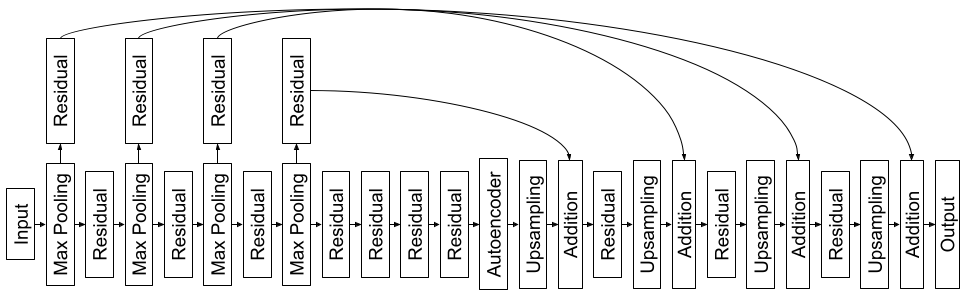
\includegraphics[width = \textwidth]{entities/SHG_AE.png}
    \caption{Visualization of the proposed combination of the hourglass and autoencoder for the stacked hourglass.}
    \label{fig:SHG_AE}
\end{figure}
\\
The autoencoder takes the output of the third residual of the bottleneck of our developed stacked hourglass as input, hence why the autoencoder will be placed after the third residual to form a new proposed hourglass for the stacked hourglass, as visualized in Figure \ref{fig:SHG_AE}.
\\
\\
The training of the new model consits of two parts to speed up the training. First the autoencoder is trained isolated. Then, the trained autoencoder is placed in the developed stacked hourglass, following the structure of Figure \ref{fig:SHG_Ae}, and the whole network is trained.
\\
\\
The autoencoder is trained using Stochastic gradient descent with Nesterov momentum, $MSE$ as the loss function and a learning rate of $5e-4$, which is halved every $25$th epoch. To increase the robustness of the autoencoder, we add noise sampled from
$$\mathcal{N} \left(0, x^2e-2 \right)$$
to each training sample, where $x$ is the value of the training sample. To help the model converge, we sample from a Glorot normal distribution, like in the case with the stacked hourglass.
\\
\\
After the autoencoder has been trained, the whole network is further trained by following Newell \textit{et al.} \cite{Newell} as described in Section \ref{subsec:conf_details}.

\subsection{Results}
\begin{figure}
    \centering
    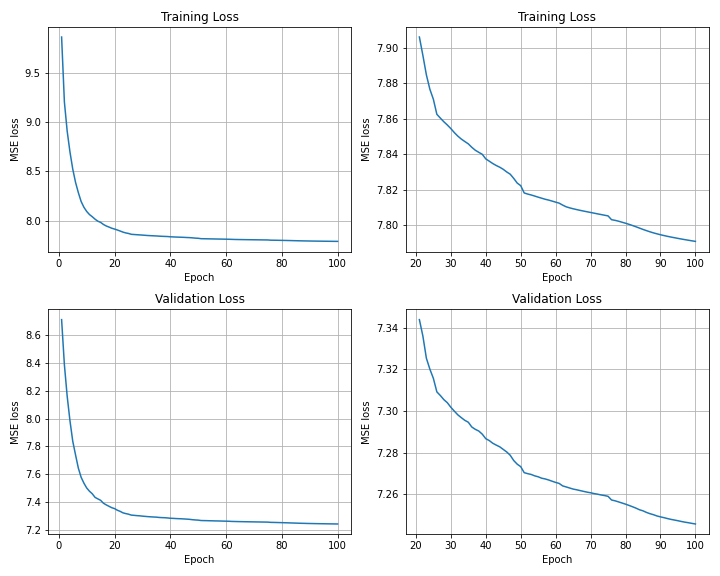
\includegraphics[height = 10 cm]{entities/AE_evolution.png}
    \caption{Visualization of the evolution of the traning- and validation loss of the trained autoencoder. The left column shows all of the $100$ epochs. Right column shows epoch $21$ and foward}
    \label{fig:AE_evolution}
\end{figure}
By training the autoencoder isolated, we get the evolution of the training- and validation loss visualized in Figure \ref{fig_AE_evolution}. We can clearly see, how the model does not start to overfit, as in the case when we trained the stacked hourglass. We decided to stop the training of the autoencoder, as each update only yielded minor changes to the model.
\\
\\
% Træning af SHG + AE resultater/plot

% Testing af SHG vs SHG + AE

% XAI af AE?


\end{document}